\documentclass{article}
%%
%% Default settings for artisynth
%%
\NeedsTeXFormat{LaTeX2e}
%%\ProvidesPackage{artisynthDoc}[2012/04/05]

\usepackage[T1]{fontenc}
\usepackage[latin1]{inputenc}
\usepackage{listings}
\usepackage{makeidx}
\usepackage{latexml}
\usepackage{graphicx}
\usepackage{framed}
\usepackage{color}

\newcommand{\pubdate}{\today}
\newcommand{\setpubdate}[1]{\renewcommand{\pubdate}{#1}}

\iflatexml
\usepackage{hyperref}
\else
%% then we are making a PDF, so include things that LaTeXML can't handle: 
%% docbook style, \RaggedRight
\usepackage{ifxetex}
\usepackage{pslatex} % fixes fonts; in particular sets a better-fitting \tt font

\usepackage[A4]{artisynth_papersize}
%\usepackage[letter]{artisynth_papersize}
\usepackage[hyperlink]{asciidoc-dblatex} 

%\usepackage{verbatim}
\usepackage{ragged2e}
\setlength{\RaggedRightRightskip}{0pt plus 4em}
\RaggedRight
\renewcommand{\DBKpubdate}{\pubdate}
\renewcommand{\DBKreleaseinfo}{}
\fi

% set hypertext links to be dark blue:
\definecolor{darkblue}{rgb}{0,0,0.8}
\definecolor{sidebar}{rgb}{0.5,0.5,0.7}
\hypersetup{colorlinks=true,urlcolor=darkblue,linkcolor=darkblue}

%%%%%%%%%%%%%%%%%%%%%%%%%%%%%%%%%%%%%%%%%%%%%%%%%%%%%%%%%%%%%%%%%%%%%%%%%%%%%
%
% Define macros for handling javadoc class and method references
%
%%%%%%%%%%%%%%%%%%%%%%%%%%%%%%%%%%%%%%%%%%%%%%%%%%%%%%%%%%%%%%%%%%%%%%%%%%%%%
\makeatletter

% code inspired by http://stackoverflow.com/questions/2457780/latex-apply-an-operation-to-every-character-in-a-string
\def\removeargs #1{\doremoveargs#1$\wholeString\unskip}
\def\doremoveargs#1#2\wholeString{\if#1$%
\else\if#1({()}\else{#1}\taketherest#2\fi\fi}
\def\taketherest#1\fi
{\fi \doremoveargs#1\wholeString}

% Note: still doesn't work properly when called on macro output ...
% i.e., \dottoslash{\concatnames{model}{base}{foo}} fails 
\def\dottoslash #1{\dodottoslash#1$\wholeString\unskip}
\def\dodottoslash#1#2\wholeString{\if#1$%
\else\if#1.{/}\else{#1}\fi\dottaketherest#2\fi}
\def\dottaketherest#1\fi{\fi \dodottoslash#1\wholeString}

% concatenates up to three class/method names together, adding '.' characters
% between them. The first and/or second argument may be empty, in which case
% the '.' is omitted. To check to see if these arguments are empty, we
% use a contruction '\if#1@@', which will return true iff #1 is empty
% (on the assumption that #1 will not contain a '@' character).
\def\concatnames
#1#2#3{\if#1@@\if#2@@#3\else #2.#3\fi\else\if#2@@#1.#3\else#1.#2.#3\fi\fi}

\newcommand{\javabase}{}
\newcommand{\setjavabase}[1]{\renewcommand{\javabase}{#1}}

\iflatexml
\newcommand{\javaclassx}[2][]{%
% Includes code to prevent an extra '.' at the front if #1 is empty. It
% works like this: if '#1' is empty, then '#1.' expands to '.', and so 
% '\if#1..' will return true, in which case we just output '#2'.
\href{@JDOCBEGIN/\concatnames{\javabase}{#1}{#2}@JDOCEND}{#2}}
\newcommand{\javaclass}[2][]{%
\href{@JDOCBEGIN/\concatnames{}{#1}{#2}@JDOCEND}{#2}}

\newcommand{\javamethodArgsx}[2][]{%
\href{@JDOCBEGIN/\concatnames{\javabase}{#1}{#2}@JDOCEND}{#2}}
\newcommand{\javamethodArgs}[2][]{%
\href{@JDOCBEGIN/\concatnames{}{#1}{#2}@JDOCEND}{#2}}
\newcommand{\javamethodAlt}[2]{%
\href{@JDOCBEGIN/\concatnames{}{}{#1}@JDOCEND}{#2}}
\newcommand{\javamethodAltx}[2]{%
\href{@JDOCBEGIN/\concatnames{\javabase}{}{#1}@JDOCEND}{#2}}

\newcommand{\javamethodNoArgsx}[2][]{%
\href{@JDOCBEGIN/\concatnames{\javabase}{#1}{#2}@JDOCEND}{\removeargs{#2}}}
\newcommand{\javamethodNoArgs}[2][]{%
\href{@JDOCBEGIN/\concatnames{}{#1}{#2}@JDOCEND}{\removeargs{#2}}}
\else
\def\javaurl{http://www.artisynth.org/doc/javadocs/}
\newcommand{\javaclassx}[2][]{{\color{darkblue}#2}}
%\href{\javaurl\dottoslash{\concatnames{\javabase}{#1}{#2}}.html}{#2}}
\newcommand{\javamethodArgsx}[2][]{{\color{darkblue}#2}}
\newcommand{\javamethodNoArgsx}[2][]{{\color{darkblue}\removeargs{#2}}}
\newcommand{\javaclass}[2][]{{\color{darkblue}#2}}
%\href{\javaurl\dottoslash{\concatnames{\javabase}{#1}{#2}}.html}{#2}}
\newcommand{\javamethodArgs}[2][]{{\color{darkblue}#2}}
\newcommand{\javamethodNoArgs}[2][]{{\color{darkblue}\removeargs{#2}}}
\newcommand{\javamethodAlt}[2]{{\color{darkblue}{#2}}}
\newcommand{\javamethodAltx}[2]{{\color{darkblue}{#2}}}
\fi

\newcommand{\javamethod}{\@ifstar\javamethodNoArgs\javamethodArgs}
\newcommand{\javamethodx}{\@ifstar\javamethodNoArgsx\javamethodArgsx}

%%%%%%%%%%%%%%%%%%%%%%%%%%%%%%%%%%%%%%%%%%%%%%%%%%%%%%%%%%%%%%%%%%%%%%%%%%%%%
%
% Define macros for sidebars
%
%%%%%%%%%%%%%%%%%%%%%%%%%%%%%%%%%%%%%%%%%%%%%%%%%%%%%%%%%%%%%%%%%%%%%%%%%%%%%

\iflatexml
\newenvironment{sideblock}{\begin{quote}}{\end{quote}}
\else
\usepackage[strict]{changepage}
\definecolor{sidebarshade}{rgb}{1.0,0.97,0.8}
\newenvironment{sideblock}{%
    \def\FrameCommand{%
    \hspace{1pt}%
    {\color{sidebar}\vrule width 2pt}%
    %{\vrule width 2pt}%
    {\color{sidebarshade}\vrule width 4pt}%
    \colorbox{sidebarshade}%
  }%
  \MakeFramed{\advance\hsize-\width\FrameRestore}%
  \noindent\hspace{-4.55pt}% disable indenting first paragraph
  \begin{adjustwidth}{}{7pt}%
  %\vspace{2pt}\vspace{2pt}%
}
{%
  \vspace{2pt}\end{adjustwidth}\endMakeFramed%
}
\fi

\iflatexml
\newenvironment{shadedregion}{%
  \definecolor{shadecolor}{rgb}{0.96,0.96,0.98}%
  \begin{shaded*}%
% Put text inside a quote to create a surrounding blockquote that
% will properly accept the color and padding attributes
  \begin{quote}%
}
{%
  \end{quote}%
  \end{shaded*}%
}
\else
\newenvironment{shadedregion}{%
  \definecolor{shadecolor}{rgb}{0.96,0.96,0.98}%
  \begin{shaded*}%
}
{%
  \end{shaded*}%
}
\fi

% Wanted to create a 'listing' environment because lstlisting is
% tedious to type and because under latexml it may need
% some massaging to get it to work properly. But hard to do
% because of the verbatim nature of listing
%\iflatexml
%\newenvironment{listing}{\begin{lstlisting}}{\end{lstlisting}}%
%\else
%\newenvironment{listing}{\begin{lstlisting}}{\end{lstlisting}}%
%\fi

\iflatexml\else
% fancyhdr was complaining that it wanted a 36pt header height ...
\setlength{\headheight}{36pt}
\fi

% abbreviation for backslash character
\newcommand\BKS{\textbackslash}


% Convenience stuff
\newcommand{\ifLaTeXMLelse}[2]{%
  \iflatexml %
  #1 %
  \else %
  #2 %
  \fi %
}

\newcommand{\ifLaTeXML}[1]{ %
  \iflatexml %
  #1 %
  \fi %
}

\makeatother


\setcounter{tocdepth}{5}
\setcounter{secnumdepth}{3}

\def\SEP{/}
\def\TOP{/}
\def\FULLSYSTEM{64-bit Linux }
\def\SYSTEM{Linux }
\def\ARCH{Linux64 }
\def\directory{directory }
\def\directories{directories }

\title{ArtiSynth Installation Guide for \SYSTEM}
\author{John Lloyd and Sebastian Kazenbroot-Guppy}
\iflatexml
\date{}
\fi

\begin{document}

\maketitle

\iflatexml{\large\today}\fi


\tableofcontents

\section{Introduction}

This document describes how to install and run ArtiSynth on \FULLSYSTEM
machines. There are two ways to obtain ArtiSynth: downloading
a prepackaged release, or checking out the latest development version
via Subversion. Downloading a prepackaged release is the easiest
solution to simply try out some of the basic demo programs. Checking
out the development version is recommended for developers who want to
keep their codebase current.

The typical install sequence looks like this:

\begin{description}

\item[Download]
Download either a release (Section \ref{PrepackagedRelease}) or 
check out the development version (Section \ref{SubversionCheckout}).

\item[Build]
Compile the system (Section \ref{Building}). This
step is not needed for prepackaged releases.

\item[Run] 
Start ArtiSynth and run the demonstration models (Section \ref{Running}).

\end{description}

Generally, users will also want to install and run external models and
packages that have been created either by others or by themselves.
This is discussed in (Section \ref{AdditionalModelsAndPackages}).

\section{Prerequisites}

To install ArtiSynth on \SYSTEM, you will need:

\begin{itemize}

\item A 64 bit version of \SYSTEM

\item Java JDK 6 or higher

\end{itemize}

Note that we have stopped supporting 32 bit systems, both because they
are becoming obsolete, and because ArtiSynth applications often
require more memory than they can provide.

For Java, the full Java development kit (JDK) is required, which comes
with the Java compiler {\tt javac}. The run time environment (JRE)
will not be sufficient. However, there is no need for extra bundles
such at JavaFX, NetBeans, or EE.

At the time of this writing, JDKs can be obtained free from Oracle at
\href{http://www.oracle.com/technetwork/java/javase/downloads/index.html}
{http://www.oracle.com/technetwork/java/javase/downloads/index.html}.
We currently recommend either JDK 7 or 6. Note that JDKs are sometimes
refered to by multiple names; for example, JDK 6 is sometimes refered
to as JDK 1.6.

In this document, the location of the ArtiSynth installation \directory
will be denoted by {\tt \$ARTISYNTH\_HOME}.  That
means that if ArtiSynth is installed in
\begin{verbatim}
  /home/roger/artisynth_core
\end{verbatim}
then {\tt \$ARTISYNTH\_HOME\SEP lib} denotes the \directory
\begin{verbatim}
  /home/roger/artisynth_core/lib
\end{verbatim}

\section{Downloading a Prepacked Release}
\label{PrepackagedRelease}

\subsection{Downloading and unpacking the zip file}

To obtain one of the packaged distributions, go to
\href{http://www.artisynth.org/downloads} 
{www.artisynth.org/downloads}
and select the distribution
you want. Download it, and unzip it in an appropriate location on your
computer.

Once ArtiSynth is downloaded and unpacked, it should be possible to
run it immediately by executing the {\tt artisynth} command located
in {\tt \$ARTISYNTH\_HOME\SEP bin} (see Section \ref{artisynthCommandLine}).

\section{Checking out from Subversion}
\label{SubversionCheckout}

The latest development version is available from Subversion. Once
checked out, users can continue to update the codebase to keep it
current (Section \ref{UpdatingArtiSynth}). Developers that we work
with closely can also obtain, by mutual arrangement, write access to
our Subversion repository, allowing them to also commit changes.

The ArtiSynth Subversion URL is
\begin{verbatim}
   http://svn.artisynth.org/repositories/artisynth_core/trunk
\end{verbatim}
There are several ways to check ArtiSynth out from this URL:

\subsection{Checking out using Eclipse}
\label{ArtiSynthEclipseCheckout}

If you are planning to develop ArtiSynth models in Java, and if you
are planning to do this with Eclipse (Section \ref{EclipseIDE}), then
it might be easiest to do the Subversion checkout directly in Eclipse.
Follow the instructions in Section \ref{importingFromSubversion},
using the ArtiSynth Subversion URL (above) as the {\it
Subversion\_url}.

\subsection{Checking out using the command line}
\label{ArtiSynthCygwinCheckout}

If your \SYSTEM distribution has Subversion installed, then you can
check out ArtiSynth using the following command:

\begin{lstlisting}
> svn co http://svn.artisynth.org/repositories/artisynth_core/trunk artisynth_core
\end{lstlisting}

This will check out ArtiSynth and place it in the specified \directory 
(in this case {\tt artisynth\_core}).

\subsection{Downloading the libraries}
\label{DownloadingLibraries}

Because the {\tt jar} files and native libraries used by ArtiSynth
are large, they are not stored in the Subversion repository.
Instead, they must be downloaded separately. This can be
done using the command {\tt updateArtisynthLibs}, located
in {\tt \$ARTISYNTH\_HOME\SEP bin}. You can execute it
from the command line like this:
\begin{verbatim}
 > cd $ARTISYNTH_HOME
 > bin/updateArtisynthLibs
\end{verbatim}

\section{Building ArtiSynth}
\label{Building}

If ArtiSynth has been obtained directly from Subversion, it will be
necessary to build (compile) it. This is not necessary for prepackaged
releases, which are pre-built, although one may want to rebuild a
release anyway for development purposes.

\subsection{Building with Eclipse}
\label{BuildingWithEclipse}

If your Subversion checkout has been done externally to Eclipse (i.e.,
not according to Section \ref{ArtiSynthEclipseCheckout}), then you
need to first import ArtiSynth into Eclipse. Follow the instructions
in Section \ref{importingArtisynth}.

Once ArtiSynth has been imported, you should be able to build it.  If
necessary, first open a Java perspective by choosing {\sf Window >
Open Perspective > Java}. The project {\tt artisynth\_core} (or
whatever you might have named it) should appear in the {\sf Package
Explorer} window. To build the system, select the project in the {\sf
Package Explorer} window, and then choose {\sf Project > Build
Project}. Note that it may be necessary to deselect {\sf Build
Automatically} in order to enable {\sf Build Project}.

\subsection{Building from the command line}
\label{BuildingWithCygwin}

ArtiSynth can also be built by running a {\tt make} command in the top
level \directory. Before doing this, you need to first set the environment
variables {\tt ARTISYNTH\_HOME} and {\tt CLASSPATH} as described in
Sections \ref{EnvironmentVariables}. ArtiSynth can then be built by
executing

\begin{verbatim}
> cd $ARTISYNTH_HOME
> make
\end{verbatim}

\section{Running ArtiSynth}
\label{Running}

\subsection{Running from the command line}
\label{artisynthCommandLine}

The most direct way to start ArtiSynth is to run the commad
{\tt \$ARTISYNTH\_HOME\SEP bin\SEP artisynth}:

\begin{verbatim}
 > cd $ARTISYNTH_HOME
 > bin/artisynth
\end{verbatim}

\subsection{Running using Eclipse}

Once ArtiSynth has been imported into Eclipse (and built if
necessary), it should contain a launch configuration called {\tt
ArtiSynth} that will allow ArtiSynth to be run.

Generally, it is first necessary set environment variables in the
launch configuration to allow ArtiSynth to find runtime configuration
files and libraries. Instructions for setting these variables are
contained in Section \ref{EclipseEnvironmentVariables}.  If the same
environment variables have already been set externally in \SYSTEM,
(Sections \ref{EnvironmentVariables}), then they do not need to be set
in the launch configuration.

Once the environment variables are set, it should be possible to run
ArtiSynth by choosing {\sf Run > Run}.

\subsection{Testing the Demo Models}

Once ArtiSynth starts up, you can try out the various demonstration
models. From the menu bar, Select {\sf Models > Demos}.  This
will display a submenu of demonstration models. Choosing one will
cause that model to be loaded and displayed in the viewer.  Simulation
of the model can then be started, paused, single-stepped, or reset
using the play controls (Figure \ref{PlayControlsFig})
located at the upper right of the ArtiSynth window frame.

\begin{figure}
\begin{center}
\iflatexml
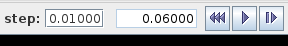
\includegraphics[]{images/playControls}
\else
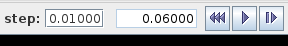
\includegraphics[width=2.5in]{images/playControls}
\fi
\end{center}
\caption{The ArtiSynth play controls. From left to right: step size
control, current simulation time, and the reset, play/pause, and
single-step buttons.}%
\label{PlayControlsFig}
\end{figure}

Comprehensive information on exploring and interacting with models is
given in the
\href{http://www.artisynth.org/doc/html/uiguide/uiguide.html}
{ArtiSynth User Interface Guide}.

\section{Installing External Models and Packages}
\label{AdditionalModelsAndPackages}

Typically, an ArtiSynth developer will want to use external models and
packages that exist outside of {\tt artisynth\_core}.  Some of these
may be obtained from external sources.  For example, {\tt
artisynth\_models} is a collection of packages, currently hosted at
{\tt www.artisynth.org/models}, that provides a variety of publicly
available anatomical models.

Installing external models and packages requires a sequence of
operations similar to that for installing ArtiSynth itself:

\begin{enumerate}

\item Download

\item Build (if necessary)

\item Run

\end{enumerate}

\subsection{Downloading}

Some model and package collections, such as {\tt artisynth\_models}
mentioned above, may be available either as prepackaged distributions
or as Subversion checkouts. Prepackaged distributions should be
downloaded and unpacked into a desired location, while Subversion
checkouts may be obtained with the {\tt svn} command as
described in Section \ref{SubversionCheckout}, using the
appropriate Subversion URL in place of the ArtiSynth Subversion URL. Some
collections maintained by ArtiSynth may contain Eclipse project
settings (in an {\tt eclipseSettings.zip} file in their root
\directory), allowing them to be imported into Eclipse, either
directly from Subversion (Section \ref{importingFromSubversion}), or
after being obtained separately (Section \ref{importingArtisynth}).

\subsection{Building}

Collections that are obtained from Subversion will need to be built
(compiled).

Those imported into Eclipse can be built as described in Section
\ref{BuildingWithEclipse}. However, in order to compile properly, the
{\tt artisynth\_core} project (and any other projects they depend on)
were have to be added to their build path. Details on doing this are
given in Section \ref{AddingProjectsToBuildPath}.

Alternatively, if the collection has a {\tt Makefile} in its root
\directory, then it can be compiled from the command line by running {\tt
make} in the root \directory. Before doing this, the top-level
\directory for the collection's {\tt class} files must to be added to
the {\tt CLASSPATH} environment variable (Sections
\ref{EnvironmentVariables}). In collections maintained by ArtiSynth,
this will be the \directory {\tt classes}, located directly under the
collection root \directory (e.g., {\tt artisynth\_models\SEP classes}).



\subsection{Running}

External models are executed by running ArtiSynth itself (Section
\ref{Running}). However, in order to execute these models, ArtiSynth
must be able to locate their associated classes. This can be
arranged in three different ways:

\subsubsection{Adding external classes using the Eclipse Classpath}

If you are running from Eclipse, then you can make the classes of
external projects visible to ArtiSynth by adding the projects to the
{\sf Classpath} of your ArtiSynth launch configuration, as described
in Section \ref{AddingProjectsToLaunch}.

\subsubsection{Adding external classes using EXTCLASSPATH}

Alternatively, you can make the classes of external projects visible
to ArtiSynth by adding the path names of all their top-level class
\directories (or {\tt jar} files, if relevant) to the file {\tt
\$ARTISYNTH\_HOME\SEP EXTCLASSPATH} (described in Section
\ref{EXTCLASSPATHFile}).

For example, suppose the collection {\tt artisynth\_models}
has been placed in {\tt \TOP projects\SEP artisynth\_models}.
The top-level class \directory for this collection is located
in {\tt artisynth\_models\SEP classes}, and so the following entry
should be placed in the {\tt EXTCLASSPATH} file:

\begin{verbatim}
/projects/artisynth_models/classes
\end{verbatim}

\subsubsection{Adding external classes using CLASSPATH}

Finally, if you are running from the command line using the {\tt
artisynth} command, then you can make external classes visible by adding
them to your {\tt CLASSPATH} environment variable (see Section
\ref{EnvironmentVariables}).

\section{Updating ArtiSynth}
\label{UpdatingArtiSynth}

One reason to use a checkout of the latest ArtiSynth
development version is to be able to migrate recent changes into your
code base. When a significant update occurs, a posting is made to the
ArtiSynth update log, currently located at
\href{http://www.artisynth.org/doc/html/updates/updates.html}
{www.artisynth.org/doc/html/updates/updates.html}.
Users may also be notified via the {\tt artisynth-updates} email list.

Users working from Eclipse with a Subversion plugin installed
(Section \ref{importingFromSubversion}) may update simply by selecting
the project in the {\sf Package Explorer} and selecting {\sf Team >
Update} from the context menu.

Updating may also be done from the command line using the {\tt svn}
command in the ArtiSynth installion \directory:
\begin{verbatim}
   cd $ARTISYNTH_HOME
   svn update 
\end{verbatim}

\subsection{Library updates}

Occasionally, a software update will be accompanied by a change in the
libraries located in {\tt \$ARTISYNTH\_HOME\SEP libs}.  When this
happens, it will be indicated on the ArtiSynth update log and
appropriate instructions will be given. Sometimes, it will be
necessary to explicitly update the libraries after doing the main
update. This can be done by executing {\tt updateArtisynthLibs} as
described in Section \ref{DownloadingLibraries}.

\section{The Eclipse IDE}
\label{EclipseIDE}

Eclipse is an integrated development environment (IDE) commonly used
for Java code development, and many ArtiSynth developers use it for
both programming models and for running the system. This section
describes how to load ArtiSynth projects into Eclipse, and how to
configure it for running ArtiSynth. A general introduction to Eclipse
is beyond the scope of this document, but there are many Eclipse
resources available online.

\subsection{Obtaining Eclipse}

Eclipse can be obtained from
\href{http://www.eclipse.org/downloads}{www.eclipse.org/downloads}.  A
good version to obtain (at the time of this writing) is {\sf Eclipse
IDE for Java Developers}.

\subsubsection{Installing a Subversion plugin}

\label{SubversionPlugIn}

In order to work with Subversion from within Eclipse, either to check
out ArtiSynth from the repository, or to update or commit changes, it
is necessary to use a Subversion plug-in. First, check to see if your
version of Eclipse contains an Subversion plug-in:

Open an import panel using {\sf File > Import...}, and then look for
{\sf SVN} in the set of available import sources. If you don't see SVN
listed, it will be necessary to install a plug-in.

We recommend the Eclipse-supported Subversive plug-in, but if this
proves difficult for any reason, there are other options, such as
Subclipse, currently obtainable from
\href{http://subclipse.tigris.org/servlets/ProjectProcess?pageID=p4wYuA}
{subclipse.tigris.org}.

Subversive can usually be installed from within Eclipse. The
recommended method is through the Eclipse Marketplace, which is
available in modern releases of Eclipse and available for previous
versions through \href{http://www.eclipse.org/mpc/}{www.eclipse.org/mpc}.

To access the Eclipse Marketplace, click {\sf Help > Eclispe}
Marketplace. Once the applications available have loaded in, type {\tt
Subversive} into the {\sf Find} box in the top-left corner of the
Marketplace window. Navigate to the package labeled {\sf Subversive -
SVN Team Provider 2.0} and click {\sf Install}. On the {\sf Confirm
Selected Features} screen, ensure all boxes are checked and click the
button labeled {\sf Confirm >}. Restart Eclipse when prompted.

If the Eclipse Marketplace is not available or desired, nagivate to
{\sf Help > Install New Software} and enter
{\tt http://download.eclipse.org/technology/subversive/2.0/update-site/}
in the text field. Check {\sf Subversive Integration Plug-in's} and
{\sf Subversion SVN Team Provider Plug-In} and click {\sf Next} and
then follow the installation instructions.

No matter how Subversive was installed, one more step is
necessary. Re-open Eclipse, and you should be prompted to choose an SVN
connector in the start menu.  SVN connectors interface
Subversive to the SVN server, and are OS and server-specific. A
recommended SVN Connector will be pre-selected for downloading; this
is most likely the one you need.

SVN connectors can also be installed separately (thanks to bmaupin at
Stackoverflow):

\begin{enumerate}

\item  Go to 
\href{http://www.polarion.com/products/svn/subversive/download.php}
{www.polarion.com/products/svn/subversive/download.php}

\item Under the latest {\sf Release}, copy the Subversive SVN
Connectors URL. The current URL for Eclipse 4.3 Kepler
is \href{http://community.polarion.com/projects/subversive/download/eclipse/3.0/kepler-site/}
{http://community.polarion.com/projects/subversive/download/eclipse/3.0/kepler-site}.

\item In Eclipse, go to {\sf Help > Install New Software...} and 
click {\sf Add...}  

\item Copy the URL for the Subversive SVN Connectors into the {\sf
Location} box and click {\sf OK}

\item Check {\sf Subversive SVN Connectors}, click {\sf Next}, and
then follow the instructions to complete installation.

\end{enumerate}

You can install multiple connectors, and then choose the one you need
by going to {\sf Windows > Preferences}, opening {\sf Team > SVN}, and
then opening the {\sf SVN Connector} tab.

For further documentation, please review the Eclipse documentation on
installing Subversive at
\href{http://www.eclipse.org/subversive/installation-instructions.php}
{www.eclipse.org/subversive/installation-instructions.php}.

\subsubsection{Importing an ArtiSynth project into Eclipse}
\label{importingArtisynth}

An ArtiSynth project can be either ArtiSynth itself, or an associated
project containing specific modeling applications. Let {\tt
\$PROJECT\_ROOT} denote the project root \directory. For ArtiSynth
itself, this will be {\tt \$ARTISYNTH\_HOME}.

\begin{enumerate}

\item From {\bf outside} Eclipse, install the Eclipse settings by
unzipping {\tt \$PROJECT\_ROOT\SEP eclipse\-Settings.zip} into {\tt
\$PROJECT\_ROOT}. This will create the files {\tt .project} and {\tt
.classpath}, along with the \directory {\tt .settings}, in {\tt
\$PROJECT\_ROOT}.  For ArtiSynth itself, it will also create the file
{\tt ArtiSynth.launch} containing the launch configuration.
  
\item From within Eclipse, choose {\sf File > Import ...}.

\item In the {\sf Import} window, select {\sf General > Existing Projects into
Workspace} and click {\sf Next}.

\item In the field {\sf Select root directory}, enter (or browse to) 
{\tt \$PROJECT\_ROOT} and then click {\sf Finish}. 

\end{enumerate}

If Eclipse complains that {\sf "No projects are found to import"}, that most
likely means that {\tt eclipseSettings.zip} was not
properly unzipped into {\tt \$PROJECT\_ROOT}.

\subsubsection{Importing an ArtiSynth project directly from Subversion}
\label{importingFromSubversion}

If Eclipse has a Subversion plug-in installed (Section
\ref{SubversionPlugIn}), you may import an ArtiSynth project by
checking it out directly from the repository located by
the project's {\it Subversion\_URL}. For the core ArtiSynth
distribution, this is 
\begin{verbatim}
   http://svn.artisynth.org/repositories/artisynth_core/trunk
\end{verbatim}
Other projects will have different URLs.

The following instructions assume the Subversive plug-in.

\begin{enumerate}

\item Choose {\sf File > Import} from the main menu, select {\sf SVN >
Project from SVN} and click {\sf Next}.

\item You now need to specify a repository location, as specified by a
{\it Subversion\_URL}.  If you've previously done an SVN checkout, a
menu will appear allowing you to select a previously used URL. If one
of these is sufficient, select it and click {\sf Next} to go to Step
4. Otherwise, select {\sf Create a new repository location} and click
{\sf Next} to enter a repository dialog. If no previous locations are
known this dialog will appear automatically.

\item If you are specifying a new location in the repository dialog:

\begin{itemize}

\item Under the {\sf General} tab, enter the {\it Subversion\_URL} in the
{\sf URL} box. If you are just checking out the trunk of the
repository (i.e., if your Subversion URL ends in {\tt /trunk}), then
you should omit the final {\tt /trunk} since this is selectable in Step 4.

\item If you are checking out a repository that is not available for
anonymous access, or if you need write access to the repository, enter
your ArtiSynth User ID and Password (which you will have obtained from
us separately) in the {\sf Authentication} section of the dialog.
You will probably want to check {\sf Save authentication} as well.

%\item If you are just checking out the trunk of the repository (i.e.,
%if your Subversion URL ends in {\tt /trunk}, as most examples in this
%guide do), then go to the {\sf Advanced} tab and uncheck {\sf Enable
%Structure Detection}.

\item Click {\sf Next}.

\end{itemize}

\item In the {\sf Select Resource} dialog, use the {\sf URL} selector
box to select the full URL to be used for the checkout. If you are
just checking out the trunk of the repository, then choose {\tt
Subversion\_URL/trunk} which should be available as a selection.

\item Click {\sf Finish}

\item In the {\sf Check Out As} dialog, select {\sf Check out as a
project with name specified}, adjust the project name if desired,
and click {\sf Next}.

\item Specify the location for the check out. If you leave {\sf Use
default workspace location} selected, this will be {\tt
workspace/project\_name}, where {\tt workspace} is the Eclipse
workspace \directory and {\tt project\_name} is the project name
selected in the previous step. Otherwise, you can specify an explicit
checkout location (which does not have to be located in the Eclipse
workspace). For ArtiSynth core checkouts, the project name is
typically {\tt artisynth\_core} and the the checkout location will
become the ArtiSynth install \directory {\tt \$ARTISYNTH\_HOME}.

\item Click {\sf Finish}.

\item If necessary, open a Java perspective by choosing {\sf Window >
Open Perspective > Java}. The project should appear in the {\sf
Package Explorer} window.

\item From {\bf outside} Eclipse, install the Eclipse settings by
unzipping {\tt \$PROJECT\_ROOT\SEP eclipse\-Settings.zip} into {\tt
\$PROJECT\_ROOT}. This will overwrite the file {\tt .project}, and
create the file {\tt .classpath}, along with the folder {\tt
.settings}, in {\tt \$PROJECT\_ROOT}.  For ArtiSynth itself, it will
also create the file {\tt ArtiSynth.launch} containing the launch
configuration.

\begin{sideblock}
Note: if unzip queries about overwriting {\tt .project}, answer [y]es.
\end{sideblock}

\item From {\bf outside} Eclipse, download
the required {\tt jar}
files and native libraries as described in Section \ref{DownloadingLibraries}.

\item Finally, load the new settings into the project by selecting the
project in the {\sf Package Explore} window and selecting {\sf
Refresh} from the context menu.

\end{enumerate}

\subsection{Configuring environment variables}
\label{EclipseEnvironmentVariables}

To run ArtiSynth from Eclipse, it is generally necessary to set certain
environment variables directly in your Eclipse launch configuration so
that ArtiSynth can locate configuration files and native library
support. Directions on setting the environment variables are given
in Section \ref{SettingEnvironmentVariables}. The required
settings are:

\begin{itemize}

\item Set {\tt ARTISYNTH\_HOME} to the path of the ArtiSynth
installation \directory.

\item Set {\tt LD\_LIBRARY\_PATH} to {\tt \$ARTISYNTH\_HOME\SEP lib\SEP \ARCH}

\item Optionally, set {\tt OMP\_NUM\_THREADS} (see Section
\ref{EnvironmentVariables}).

\item Optionally, set {\tt ARTISYNTH\_PATH} 
(see Section \ref{EnvironmentVariables}).

\end{itemize}

If any of the above variables have already been set externally in
\SYSTEM (Section \ref{EnvironmentVariables}), then they do not need to
be set in the launch configuration.

\begin{sideblock}
{\bf Note:} At present, eclipse does not expand environment variables.
In all the variable settings described below, references to {\tt
\$ARTISYNTH\_HOME} should be expanded (manually) to the path of the
ArtiSynth install \directory.
\end{sideblock}

\subsubsection {Setting environment variables}
\label{SettingEnvironmentVariables}

To set environment variables within Eclipse:

\begin{enumerate}

\item Open a java perspective if necessary by choosing
  {\sf Window > Open Perspective > Java}.

\item Select the ArtiSynth project in the {\sf Package Explorer} form.

\item Choose {\sf Run > Run Configurations...} to open the {\sf Run
  Configurations} window.

\item In the left panel, under {\sf Java Application}, select {\sf ArtiSynth}.

\item In the right panel, select the {\sf environment} tab.

\item To create a new environment variable, click the {\sf New} button and
  enter the name and value in the dialog box.

\item When finished, make sure that {\sf Append environment to native
  environment} is selected, and click {\sf Apply}.

\end{enumerate}

\subsection{Adding projects to the build path}
\label{AddingProjectsToBuildPath}

A project imported into Eclipse may depend on the packages and
libraries found in other projects to compile properly.  For example,
ArtiSynth applications which are external to {\tt artisynth\_core}
will nonetheless depend on {\tt artisynth\_core}. To ensure
proper compilation, project dependencies should be added
to each dependent project's build path.

\begin{enumerate}

\item Select the dependent project in the {\sf Package Explorer} form.

\item Right click and choose {\sf Build Path > Configure Build Path...} 

\item In the right panel, select the {\sf Projects} tab.

\item Click the {\sf Add} button, select the project dependencies,
      and click {\sf OK}

\item Click {\sf OK} in the Java Build Path panel

\end{enumerate}

\subsection{Adding projects to the ArtiSynth launch configuration}
\label{AddingProjectsToLaunch}

The classes of external projects can be made visible to ArtiSynth by
adding the projects to the Classpath of the ArtiSynth launch
configuration.

\begin{enumerate}

\item From the main menu, choose {\sf Run > Run Configurations...}
to open a {\sf Run Configurations} dialog.

\item In the left panel, under {\sf Java Application}, select your
ArtiSynth launch configuration (the default one is called {\sf
ArtiSynth}). This may already be selected when you open the panel.

\item In the right panel, select the {\sf Classpath} tab.

\item In the {\sf Classpath:} window, select {\sf User Entries},
and then click the {\sf Add Projects} button.

\item In the {\sf Project Selection} dialog, select the external
projects that you wish to add. Generally, the boxes
{\sf Add exported entries ...} and {\sf Add required projects ...}
can be unchecked. Click {\sf OK}.

\item Close the {\sf Run Configurations} dialog.

\end{enumerate}

\subsection{Preventing excessive resource copying}

By default, ArtiSynth classes are built in a \directory tree ({\tt
\$PROJECT\_ROOT\SEP classes}) that is separate from the source tree ({\tt
\$PROJECT\_ROOT\SEP src}), where {\tt \$PROJECT\_ROOT} denotes the project
root \directory and is {\tt \$ARTISYNTH\_HOME} for ArtiSynth itself.
That means that Eclipse will try to copy all non-Java files and
\directories from the source tree into the build tree. For ArtiSynth,
this is excessive, and results in many files being copied that don't
need to be, since ArtiSynth looks for resources in the source tree
anyway.

On MacOS and Linux, you can inhibit most of this copying:

\begin{enumerate}

\item Choose {\sf Window > Preferences} (or {\sf Eclipse > Preferences}).

\item Select {\sf Java > Compiler > Building}.

\item Open {\sf Output directory}, and in the box entitled {\sf Filter resources},
  enter the string:

\begin{lstlisting}
    Makefile,*.l*,*.?,*.??,*.???,*.????,???,????,?????
\end{lstlisting}

\end{enumerate}

That should filter out the copying of most non-java files.

Or, to prevent copying any resource, simply enter: 
\begin{lstlisting}
    *
\end{lstlisting}

\section{Additional Information}

\subsection{Environment variables}
\label{EnvironmentVariables}

This is a glossary of all the environment variables that are
associated with building or running ArtiSynth. Often, the system can
detect and set appropriate values for these automatically. In other
cases, as noted in the above documentation, it may be necessary or
desirable for the user to set them explicity.

\begin{description}

\item[ARTISYNTH\_HOME]\mbox{}
 
The path name of the ArtiSynth installation \directory.

\item[ARTISYNTH\_PATH]\mbox{}

A list of \directories, separated by colons ":", which ArtiSynth
uses to search for configuration files such as {\tt .artisyntInit} or
{\tt .demoModels}.  A typical setting for {\tt ARTISYNTH\_PATH}
consists of the current \directory (indicated by "{\tt .}"), the user's
home \directory, and the ArtiSynth installation \directory. If {\tt
ARTISYNTH\_PATH} is not defined explicitly in the user's environment,
ArtiSynth assumes an implicit path consisting of the \directory
sequence just described.

\item[CLASSPATH]\mbox{}

A list of \directories and/or {\tt jar} files, separated by
colons ":", which Java uses to locate its class files. This
variable should be set to include {\tt \$ARTISYNTH\_HOME\SEP classes}
and {\tt \$ARTISYNTH\_HOME\SEP lib\SEP *} (the latter uses the
wildcard {\tt *} to specify all the {\tt jar} files in {\tt
\$ARTISYNTH\_HOME\SEP lib}).

\item[PATH]\mbox{}
 
A list of \directories, separated by colons ":", which the
operating system uses to locate executable programs and
applications. This should be set to include {\tt \$ARTISYNTH\_HOME\SEP bin}
and {\tt \$ARTISYNTH\_HOME\SEP lib\SEP \ARCH}.

\item[LD\_LIBRARY\_PATH]\mbox{}

A list of \directories, separated by colons
":", which the operating system searches in order to find shared libraries.
Should be set to include {\tt \$ARTISYNTH\_HOME\SEP lib\SEP \ARCH}.

\item[OMP\_NUM\_THREADS]\mbox{}
 
Specifies the maximum number of processor cores that are available for
multicore execution. Setting this variable to the maximum number of
cores on your machine can significantly increase performance.

\end{description}

%JYTHON\_HOME::
%If Jython is installed on the system, should be set to the name of the
%Jython installation \directory.

Note that settings for most of the above can be derived from the value
of {\tt ARTISYNTH\_HOME}.

\subsubsection{Example environment set up for {\tt bash}}
\label{BashEnvironmentSetup}

If you are using {\tt bash} as your shell, then the environment can be
configured by placing a block of commands similar to the following in
one of your {\tt bash} initialization files (typically {\tt
\textasciitilde/.bashrc}), located in your home \directory:

\begin{lstlisting}
# set ARTISYNTH_HOME to the appropriate location ...
export ARTISYNTH_HOME=$HOME/artisynth_2_X
export ARTISYNTH_PATH=.:$HOME:$ARTISYNTH_HOME
export LD_LIBRARY_PATH=$ARTISYNTH_HOME/lib/Linux64:$LD_LIBRARY_PATH
export CLASSPATH=$ARTISYNTH_HOME/classes:$ARTISYNTH_HOME/lib/'*':$CLASSPATH
export PATH=$ARTISYNTH_HOME/bin:$PATH
# Set to the number of cores on your machine:
export OMP_NUM_THREADS=2 
\end{lstlisting}

Be sure to set {\tt ARTISYNTH\_HOME} to the proper location of your
ArtiSynth installation \directory.

These environment variables will be passed on to any program which you
run from the shell (such as {\tt artisynth} or {\tt eclipse}).

Alternatively, you can source the script {\tt setup.bash}, located in
the installation \directory:

\begin{verbatim}
 > source setup.bash
\end{verbatim}

This will determine the system type automatically and set the
environment variables accordingly, with {\tt ARTISYNTH\_HOME} set to the
current \directory from which the script is called (however,
it {\it won't} set {\tt OMP\_NUM\_THREADS}).

\subsection{Example environment setup for {\tt csh} or {\tt tcsh}}
\label{CshEnvironmentSetup}

If you are using {\tt csh} or {\tt tcsh} as your shell, then the
environment can be configured by placing a block of commands similar
to the following in your {\tt .cshrc} file, located in your home
\directory:

\begin{lstlisting}
# set ARTISYNTH_HOME to the appropriate location ...
setenv ARTISYNTH_HOME $HOME/artisynth_2_X
setenv ARTISYNTH_PATH .":"$HOME":"$ARTISYNTH_HOME
setenv LD_LIBRARY_PATH $ARTISYNTH_HOME/lib/Linux64":"$LD_LIBRARY_PATH
setenv CLASSPATH "$ARTISYNTH_HOME/classes:$ARTISYNTH_HOME/lib/*:$CLASSPATH"
setenv PATH $ARTISYNTH_HOME/bin":"$PATH
# Set to the number of cores on your machine:
setenv OMP_NUM_THREADS 2 
\end{lstlisting}

These environment variables will be passed on to any program which you
run from the shell (such as {\tt artisynth} or {\tt eclipse}). 

Alternatively, you can source the script {\tt setup.csh}, located in
the installation \directory:

\begin{verbatim}
 > source setup.csh
\end{verbatim}

This will determine the system type automatically and set the
environment variables accordingly, with {\tt ARTISYNTH\_HOME} set to the
current \directory from which the script is called (however,
it {\it won't} set {\tt OMP\_NUM\_THREADS}).

\subsection{ArtiSynth Libraries}

ArtiSynth uses a set of libraries located under {\tt
\$ARTISYNTH\_HOME\SEP lib}. These include a number of {\tt jar} files,
plus native libraries located in architecture-specific sub-\directories
({\tt \ARCH} for \FULLSYSTEM systems).

As described in Section \ref{DownloadingLibraries}, these libraries
need to be downloaded automatically if the system is obtained from the
Subversion repository. The required libraries are listed in the file
{\tt \$ARTISYNTH\_HOME\SEP lib\SEP LIBRARIES}. This file is checked
into the repository, so that the system can always determine what
libraries are needed for a particular checkout version.

Occasionally the libraries are changed or upgraded.  If you run
ArtiSynth with the {\tt -updateLibs} command line option, the program
will ensure that not only are all the required libraries present, but
that they also match the latest versions on the ArtiSynth server.

\subsection{The EXTCLASSPATH File}
\label{EXTCLASSPATHFile}

In order to run an external model or package in ArtiSynth, all class
paths (i.e., class \directories or {\tt jar} files) associated with
those external classes must be made known to ArtiSynth. This is done
by listing these class paths as entries in the text file {\tt
EXTCLASSPATH}, located in {\tt \$ARTISYNTH\_HOME}.

To add class paths to {\tt EXTCLASSPATH}, open it using a standard
text editor (such as {\tt vim}, {\tt gedit}, or {\tt emacs}), and add
each path on a separate line. (Strictly speaking, paths only need to
be separated by whitespace, but placing each on a separate line should
make the file more readable.)

The syntax rules for {\tt EXTCLASSPATH} are:

\begin{enumerate}

\item Class path entries should be separated by white space.

\item Paths containing spaces should be placed inside double quotes
({\tt "}).

\item The {\tt \#} character is a comment character.

\item The {\tt \$} character can be used to expand environment variables.

\end{enumerate}

An example {\tt EXTCLASSPATH} might look like this:

\begin{verbatim}
/research/artisynth_models/classes
/research/models/special.jar
$HOME/projects/crazy/classes
\end{verbatim}

\end{document}


%To obtain one of the packaged distributions:
%
%\begin{enumerate}
%
%\item Go to \href{http://www.artisynth.org}{http://www.artisynth.org}
%
%\item Select {\sf Software/Downloads}. This will bring up a page directing you 
%to the {\sf ArtiSynth Download Form}.
%
%\item Select the link to the {\sf ArtiSynth Download Form}.
%
%\item Fill in and submit this form. An email containing a link and a password 
%will automatically be sent to the e-mail address you provide in this form.
%
%\item Open the e-mail mentioned above and click on the given link to find a 
%password protected webpage.
%
%\item Enter the password provided by the email. Take care that no spaces are 
%included, as the system is sensitive to them.
%
%\item This will lead to a different webpage, with links to various ArtiSynth 
%distributions. Select any one to download, and click it.
%
%\item Download the distribution, and unzip it in an appropriate
%location on your computer.
%
%\end{enumerate}
